\documentclass[12pt]{article}
\usepackage{graphicx}
\usepackage{wrapfig}
\usepackage{subfigure}
\usepackage{multirow}
\usepackage{hyperref}
\usepackage{amsmath}
\usepackage{amssymb}
%\usepackage{ngerman}
\usepackage[ansinew]{inputenc}
\usepackage[left=2cm,top=1cm]{geometry}

% vector graphics test
\usepackage{color}
\usepackage{transparent}
\graphicspath{{graphs/}}

\setlength{\parindent}{0pt}

%\usepackage[outdir=./]{epstopdf}
%\epstopdfsetup{outdir=./}


\begin{document}
	\pagestyle{empty}
	\textasciitilde

\begin{titlepage}
	\centering
	\bigskip
	\huge{Astronomisches Praktikum: Altersbestimmung offener Sternhaufen}\\
	\bigskip
	\large{Versuch 4}\\
	\bigskip
	\large{Jan R\"{o}der \& Julia Lienert}
	\bigskip
	\tableofcontents
\end{titlepage}

\pagebreak


\section{Einleitung}

\section{Analyse eines unbekannten Sternhaufens}

\subsection{Aufgabe 1}

\begin{figure} [h]
	\centering
	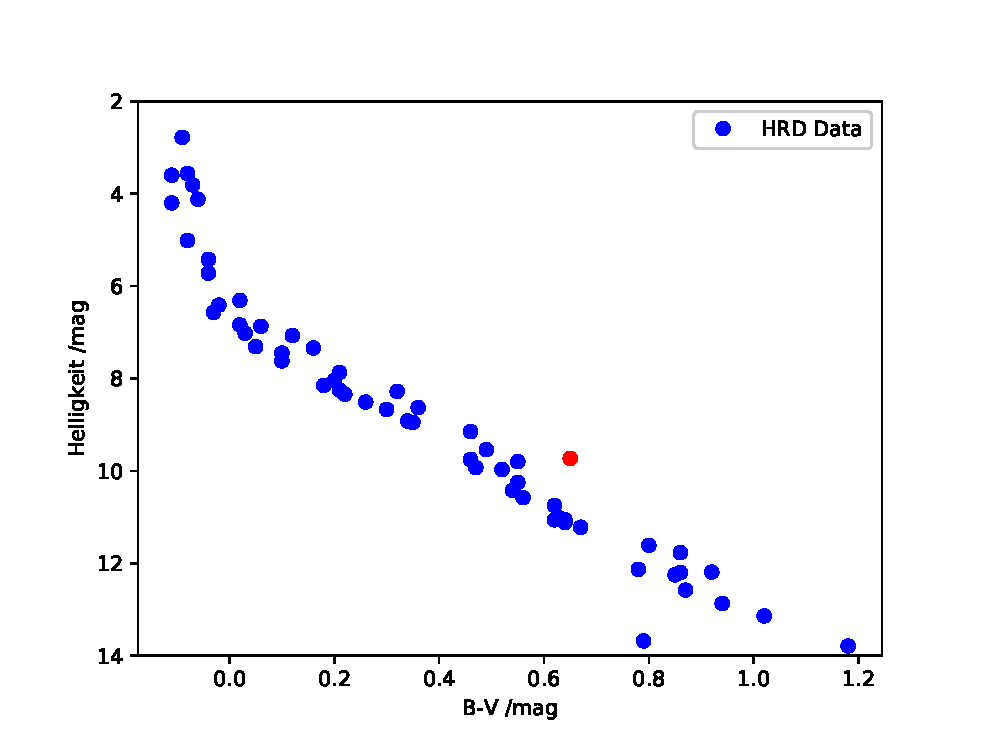
\includegraphics[width=1\textwidth]{hrd_notitle.eps}
	\caption{Scheinbare Helligkeit und Farbindex gegeneinander aufgetragen}
	\label{fig:hrd_unknown}
\end{figure}

Im Diagramm sind die Werte aus Tabelle 4.1 der Anleitung aufgetragen. Die Hauptreihe knickt bei ca. $m=5$\,mag und $B-V=-0.01$\,mag ab.

\subsection{Aufgabe 2}

Abbildung 4.2 der Anleitung zeigt die abolute Helligkeit aufgetragen gegen den Farbindex, f\"{u}r einige bekannte Sternhaufen. Hier kann man anhand des Farbindexes das ALter des unbekannten Sternhaufens ablesen. Alternativ kann der Farbindex in die effektive Temperatur umgerechnet werden, um Abbildung 4.3 b) verwenden zu k\"{o}nnen. Ohne Information \"{u}ber die Entfernung des Haufens k\"{o}nnen die y-Achsen der Graphen, die jeweils die abolute Helligkeit darstellen, nicht verwendet werden. \\
Die hellsten Sterne sind oft blaue Riesensterne, die eine Farbe zwischen wei"slichem Blau und Blau haben. Das entspricht einem Farbindex von etwa $-0.2$.

\subsection{Aufgabe 3}

Der Abknickpunkt f\"{u}r $B-V\simeq -0.01$\,mag steht hier f\'{u}r ein Alter von etwa $10^8$ Jahren (Plejaden in Abb. 4.2). 

\subsection{Aufgabe 4}

Liest man in Abb. 4.2 die zum bestimmten Farbindex geh�rende abolute Helligkeit ab, kann man sie zusammen mit der scheinbare Helligkeit des Abknickpunkts in das Entfernungsmodul einsetzen. Man erh�lt aus der Abbildung $M\simeq-0.5$\,mag.
\begin{align*}
	r &= 10\text{\,pc} \cdot 10^{\frac{m-M}{5}} \\
	r &= 10\text{\,pc} \cdot 10^{\frac{5.5}{5}} \\
	r &\simeq 125.89\text{\,pc} 
\end{align*}

\subsection{Aufgabe 5}

Das Alter von $10^8$ Jahren ergibt $\log t = 8$, mithilfe von Abbildung 4.3 b) erh�lt man dann $\log \,T_{eff}=4.1$ (der x-Wert zum Abknickpunkt der Kurve, die zu $\log t = 8$ geh�rt.) Damit ist $T_{eff} \simeq 12590$\,K. Dies wiederum liefert den x-Wert zu der Kurve zum gesuchten $\log M/M_\odot$ in Abbildung 4.3 a). Man kann $\log M/M_\odot = 0.6$ ablesen, bzw. $M\simeq3.98$\,M$_\odot$.

\subsection{Aufgabe 6}


\section{Hertzsprung-Russell-Diagramme}


\end{document}